The network metering with Zabbix is not only used for network managing  decisions. I is also possible for each user of the Smart Filesystem to get informations concerning his used energy and eventually his created costs.
\subsection{A Cost Request}
 The idea is, that each user can go on a website put a request for his account over a special time. The starting procedure is shown in figure bla. \todo{ref tikz}
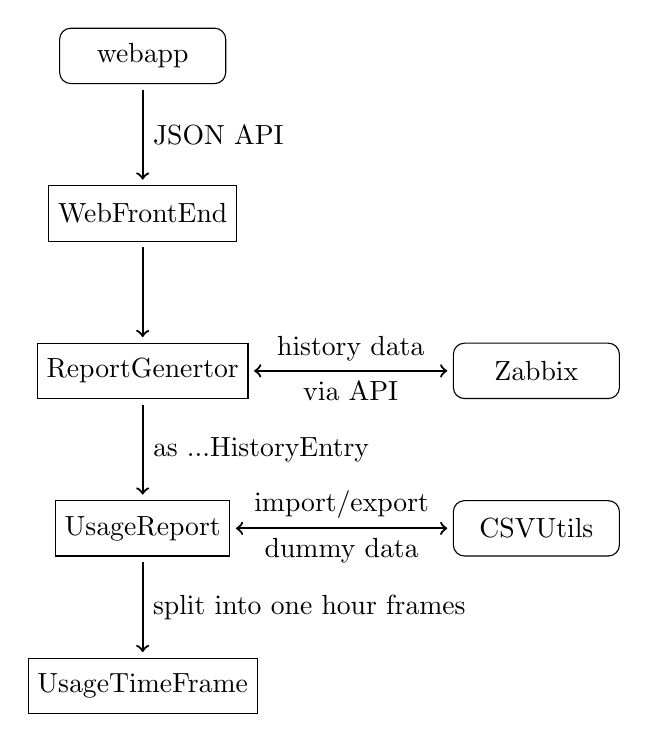
\begin{tikzpicture}
    \tikzset{
        external/.style = {
            rectangle, rounded corners, draw=black,
            minimum width=6em, minimum height=2em, text centered, node distance=5cm
        },
        internal/.style = {
            rectangle, draw=black,
            minimum width=6em, minimum height=2em, text centered, node distance=2cm
        },
        edge/.style = {
            ->, thick, shorten <= 2pt, shorten >= 2pt
        },
        dotted box/.style = {
            rectangle, draw = black, rounded corners, dashed, inner sep=3pt
        }
    };

	\node[internal] (generator) {ReportGenertor};
	\node[internal] (web) [above of = generator] {WebFrontEnd};
	\node[external, node distance = 2cm] (webapp) [above of = web] {webapp};
	\node[external] (zabbix) [right of = generator]  {Zabbix};
	\node[internal] (report) [below of = generator] {UsageReport};
	\node[external] (csv) [right of = report] {CSVUtils};
	\node[internal] (frame) [below of = report]{UsageTimeFrame};

	\draw[edge] (webapp) -- (web) node [midway, right] {JSON API};
	\draw[edge] (web) -- (generator);
	\draw[edge, <->] (generator) -- (zabbix)
		node [midway, above] {history data}
		node [midway, below] {via API};
	
	\draw[edge, <->] (report) -- (csv) 
		node [midway, above] {import/export} 
		node [midway, below] {dummy data};
	
	\draw[edge] (generator) -- (report)
		node [midway, right] {as ...HistoryEntry};
	\draw[edge] (report) -- (frame) 
		node [midway, right] {split into one hour frames};
\end{tikzpicture}

 The request goes to the "ReportGenerator" which uses the account of the user and the given time frame to create a API request for Zabbix. Zabbix gets all information about the user in the given time frame from its database and sends it back to the ReportGenerator. Now these information will be packed as so called "HistoryEntries" and forwarded to an instance of the "UsageReport" class. 
 
 This instance can import or export the data as files or starts the price calculation. To do that the UsageReport splits the data in one hour frames. This is possible because Zabbix stores for each data the time as well. These calculations will be made by the "UsageTimeFrame". After that the system can tell the uses how much he has to pay for the given time by listing the usage in one hour parts.
 
 \subsection{Calculation of the price} 
 The basic idea of the price concept is that the owners of the system do not have to pay for the maintenance of the system. Every user has pay a part of the energy usage if the severs run in idle mode as well as the user has to pay for his traffic. It should be noticed that this basic idea was made by the team. It can't work if just a few persons uses the system. On the other hand is the idea of distributed file systems that a lot of people use them. But it was not possibly to test that concept because there simply were not that much people to test that. 
 
 If we want to compute the price for each user and each system in an hour, the first thing to is to extend the data from Zabbix. Firstly Zabbix stores engery usage of each sever every two seconds. Secondly, if there is a traffic flow, Zabbix will store information about that every five seconds. And last but not least 